\chapter{双原子分子的分子轨道}\label{ch:b2:diatomic-mos}

将液氧倒入强磁铁的两磁极之间，液流被拉向一侧；
液氮则笔直落下。氧分子带有未成对电子，
磁场会吸引它们。其路易斯结构
\ce{O=O} 中所有电子都已成对，无法体现这一点。分子轨道
由上一章的原子轨道构造而成，使分子中的每个电子
各占一个能级：它们解释了氧的磁性、
化学键的强度与键长，以及使分子电离所需的
能量——并为
后续各章的反应活性奠定基础。

\begin{recall}
参见\Cref{ch:b2:atomic-orbitals}：原子轨道、其形状、
符号与能量。本科一年级分册中的路易斯结构，作为描述性概念的 $\sigma$ 键与 $\pi$ 键，
杂化及其局限，未成对电子与
自由基。
\end{recall}

\begin{omfigure}
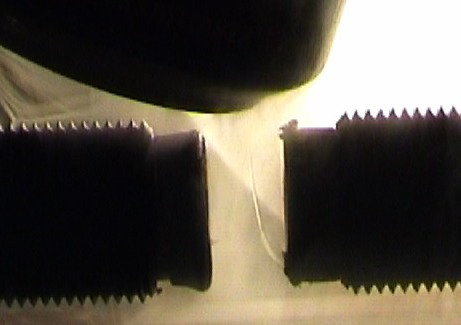
\includegraphics[width=0.42\linewidth]{images/book3/liquid-oxygen.jpg}

{\small 一股细长的液氧流落入强磁铁的两极之间，
被吸向两极并悬挂成桥状：该分子是顺磁性的。
（照片：Pieter Kuiper，公有领域，维基共享资源。）}
\end{omfigure}

\section{LCAO 方法}

\begin{definition}[分子轨道]\label{def:b2:diatomic-mos:lcao}
分子中某一个电子的波函数，分布于该分子的所有原子核之间，称为\emph{分子轨道}\index{分子轨道}。
在\emph{LCAO}\index{LCAO}
方法（原子轨道线性组合）中，它被写成各原子轨道的和，
$\psi = \sum_i c_i\varphi_i$，其中系数的选取使
能量最低。
\end{definition}

对于两个原子 A 与 B，各提供一个轨道，$\psi = c_A\varphi_A + c_B\varphi_B$。
$\psi$ 中电子的能量，关于系数求极小后，
涉及三个数。

\begin{definition}[LCAO 方法的积分]\label{def:b2:diatomic-mos:integrals}
设两个实原子轨道 $\varphi_A$、$\varphi_B$ 以及
分子中电子的能量算符 $\hat H$：
\begin{itemize}
  \item \emph{重叠积分}\index{重叠积分} $S = \int\varphi_A\varphi_B\,dV$，
        度量两个轨道占据同一区域的程度（对于
        全同、完全叠合的轨道，$S = 1$）；
  \item \emph{库仑积分}\index{库仑积分} $\alpha_A = \int\varphi_A\hat
        H\varphi_A\,dV$，是分子中处于 $\varphi_A$ 的电子的能量，
        与原子轨道能量接近；
  \item \emph{共振积分}\index{共振积分} $\beta = \int\varphi_A\hat
        H\varphi_B\,dV$，取负值，度量两个轨道的耦合强度；
\end{itemize}
分子轨道的能量 $E$ 为\emph{久期
行列式}\index{久期行列式}的根：
\[
  \begin{vmatrix} \alpha_A - E & \beta - ES \\ \beta - ES & \alpha_B - E \end{vmatrix} = 0 .
\]
\end{definition}

行列式由对 $E = \int\psi\hat H\psi\,dV/\int\psi^2\,dV$ 求极小得到，
关于 $c_A$ 与 $c_B$，两个条件 $\partial E/\partial c_A =
\partial E/\partial c_B = 0$ 构成一个齐次线性方程组，它
只有当其行列式为零时才有非零解。这一变分步骤
在此不加证明地承认。

\begin{theorem}[两个全同轨道]\label{thm:b2:diatomic-mos:homonuclear}
对于 $\alpha_A = \alpha_B = \alpha$，两个分子轨道为
\[
  E_+ = \frac{\alpha + \beta}{1 + S}, \quad \psi_+ = \frac{\varphi_A + \varphi_B}{\sqrt{2(1 + S)}} ;
  \qquad
  E_- = \frac{\alpha - \beta}{1 - S}, \quad \psi_- = \frac{\varphi_A - \varphi_B}{\sqrt{2(1 - S)}} .
\]
\end{theorem}

\begin{proof}
由行列式得 $(\alpha - E)^2 = (\beta - ES)^2$，故 $\alpha - E = \pm(\beta - ES)$。
取正号时，$E(1 + S) = \alpha + \beta$；取负号时，$E(1 - S) = \alpha
- \beta$。代回线性方程组，$(\alpha - E)c_A + (\beta - ES)c_B = 0$ 给出 $c_B
= c_A$ 对于 $E_+$，$c_B = -c_A$ 对于 $E_-$。归一化：$\int(\varphi_A \pm
\varphi_B)^2\,dV = 2 \pm 2S$。
\end{proof}

\begin{definition}[成键轨道与反键轨道]\label{def:b2:diatomic-mos:bonding}
\emph{成键轨道}\index{成键轨道}的能量低于它所组成的原子轨道：
其电子密度聚集在两核之间。
\emph{反键轨道}\index{反键轨道}的能量高于原子轨道，并在
两核之间具有一个节面。\emph{非键轨道}\index{非键轨道}
保持原子轨道的能量，因为它找不到
可与之组合的伙伴。
\end{definition}

\begin{proposition}[反键轨道升高得更多]\label{prop:b2:diatomic-mos:asymmetry}
当 $S > 0$ 时，反键能级被抬高到 $\alpha$ 之上的幅度
大于成键能级被压低到其下的幅度。
\end{proposition}

\begin{proof}
$E_+ - \alpha = (\beta - \alpha S)/(1 + S)$，$E_- - \alpha = -(\beta - \alpha S)/(1 - S)$。
分子 $\beta - \alpha S$ 为负（耦合占主导），且 $1 - S < 1
+ S$：第二个位移的绝对值更大。
\end{proof}

对于 \ce{H2}，两个电子都进入 $\psi_+$，分子
比分离的原子更稳定。对于 \ce{He2}，四个电子中有两个必须进入 $\psi_-$，
这一代价大于 $\psi_+$ 带来的收益，\ce{He2} 不能成键。

\begin{omfigure}
\begin{MOdiagram}[names, labels]
  \atom[H]{left}{ 1s = {0;up} }
  \atom[H]{right}{ 1s = {0;up} }
  \molecule[\ce{H2}]{ 1sMO = {.75;pair} }
\end{MOdiagram}
\hspace{1.5cm}
\begin{MOdiagram}[names, labels]
  \atom[He]{left}{ 1s = {0;pair} }
  \atom[He]{right}{ 1s = {0;pair} }
  \molecule[\ce{He2}]{ 1sMO = {.75;pair,pair} }
\end{MOdiagram}

{\small 图示 \ce{H2}（键级 1）与 \ce{He2}（键级 0，不成键）的分子轨道图。
每个方框表示一个能级，至多容纳两个自旋相反的电子；
虚线将每个分子轨道与构成它的原子轨道相连，
即该分子轨道由这些原子轨道组合而成。}
\end{omfigure}

\section{重叠与对称性}

\begin{definition}[$\sigma$ 轨道与 $\pi$ 轨道]\label{def:b2:diatomic-mos:sigma-pi}
直线型分子的\emph{$\sigma$ 轨道}\index{$\sigma$ 轨道}在绕分子轴的任意旋转下保持不变，
即不含包含该轴的节面。
\emph{$\pi$ 轨道}\index{$\pi$ 轨道}在绕该轴旋转 $180^\circ$ 时
变号，即含一个包含该轴的节面。星号标记反键轨道
（$\sigma^*$、$\pi^*$）。
\end{definition}

\begin{proposition}[对称性引起的零重叠]\label{prop:b2:diatomic-mos:symmetry}
若两个轨道中，一个关于包含分子轴的平面对称，
另一个则反对称，二者的重叠积分与共振积分均为零，
即二者不能组合。
\end{proposition}

\begin{proof}
关于该平面作反射时，空间不变，但乘积
$\varphi_A\varphi_B$ 在镜像点处变号，因此空间两半对
$\int\varphi_A\varphi_B\,dV$ 的贡献相互抵消。同理对
$\int\varphi_A\hat H\varphi_B\,dV$ 亦然，因为 $\hat H$ 具有分子的对称性。
\end{proof}

两个轨道若对称性相同（重叠不为零）、
重叠良好，且能量相近，则相互作用强。一个原子的 1s 轨道与另一原子的
$2\mathrm p_x$ 轨道（$x$ 垂直于轴）不能组合；
沿轴的 $2\mathrm p_z$ 轨道形成 $\sigma$ 轨道；$2\mathrm p_x$ 与
$2\mathrm p_y$ 形成两对能量相等的 $\pi$ 轨道。

\begin{omfigure}
\begin{tikzpicture}[font=\small]
  % sigma 1s
  \pic at (0,0) {oms={0.85}}; \pic at (0.7,0) {oms={0.85}};
  \node at (0.35,-0.75) {$\sigma_{1s}$};
  \pic at (2.2,0) {oms={0.85}}; \pic at (2.9,0) {oms={-0.85}};
  \node at (2.55,-0.75) {$\sigma^*_{1s}$};
  % sigma 2p
  \pic at (4.6,0) {omp={-1}{0}}; \pic at (5.6,0) {omp={1}{0}};
  \node at (5.1,-0.75) {$\sigma_{2p}$};
  \pic at (7.4,0) {omp={-1}{0}}; \pic at (8.6,0) {omp={-1}{0}};
  \node at (8.0,-0.75) {$\sigma^*_{2p}$};
  % pi 2p
  \pic at (10.2,0) {omp={1}{90}}; \pic at (10.9,0) {omp={1}{90}};
  \node at (10.55,-0.95) {$\pi_{2p}$};
  \pic at (12.2,0) {omp={1}{90}}; \pic at (12.9,0) {omp={-1}{90}};
  \node at (12.55,-0.95) {$\pi^*_{2p}$};
  \draw[black!40, dashed] (-0.6,0) -- (13.4,0);
\end{tikzpicture}

{\small 同核双原子分子的分子轨道示意图（分子轴为水平虚线）。
同相组合（成键）在两核之间聚集同色，
反相组合（反键）则在两核之间设置一个节面。
$\sigma$ 轨道关于轴对称；每个 $\pi$
轨道的节面都包含该轴。}
\end{omfigure}

\section{第二周期同核双原子分子}

两个第二周期原子的 2s 与 2p 轨道共可形成八个分子轨道，
分别为 $\sigma_{2s}$、$\sigma^*_{2s}$、$\sigma_{2p}$、两个 $\pi_{2p}$、两个 $\pi^*_{2p}$、
$\sigma^*_{2p}$。

\begin{proposition}[s--p 混合]\label{prop:b2:diatomic-mos:sp-mixing}
对 \ce{O2} 与 \ce{F2}，能级次序为 $\sigma_{2s} < \sigma^*_{2s} < \sigma_{2p} < \pi_{2p} <
\pi^*_{2p} < \sigma^*_{2p}$。对 \ce{Li2} 至 \ce{N2}，其 2s 与 2p 能级较为接近，
$\sigma$ 轨道（由 2s 与 $2\mathrm p_z$ 构成）发生混合，$\sigma_{2p}$ 被推高至
高于 $\pi_{2p}$。
\end{proposition}

\begin{proof}[论证]
$\sigma_{2s}$ 与 $\sigma_{2p}$ 轨道对称性相同，可以
相互组合。对称性相同的两个能级会相互排斥（参见下文\cref{thm:b2:diatomic-mos:heteronuclear}）：
$\sigma_{2s}$ 下降，$\sigma_{2p}$ 上升，二者越接近，效应越明显。
2s--2p 间隔沿周期增大，因此该效应在左侧较大，
而在氧与氟处较小。氮与氧之间的能级交叉
依据实测光电子能谱，在本阶段不加证明地承认。
\end{proof}

\begin{definition}[键级]\label{def:b2:diatomic-mos:bond-order}
双原子分子的\emph{键级}\index{键级}为 $b = (n_b -
n_a)/2$，其中 $n_b$ 与 $n_a$ 分别为成键
轨道与反键轨道中的电子数。
\end{definition}

\begin{proposition}[键级与键]\label{prop:b2:diatomic-mos:bond-order}
对于同一对元素的原子，键级越高，
键长越短、键越强；键级为零表示不成键。
\end{proposition}

\begin{proof}[论证]
每个成键电子在两核之间增加电子密度并降低能量；
每个反键电子则减少该密度，并使能量至少升高同样多，
（见\cref{prop:b2:diatomic-mos:asymmetry}）。净成键电子对数
衡量结合的强弱。比较仅对相似的原子有意义：\ce{Li2} 的键级为 1，与 \ce{F2} 相同，
但其 2s 轨道要大得多。
\end{proof}

\begin{definition}[顺磁性与抗磁性]\label{def:b2:diatomic-mos:magnetism}
若一种物质的分子含有未成对电子，则称其为\emph{顺磁性}\index{顺磁性}物质：
它会被吸入磁场。
若其所有电子均已成对，则称其为\emph{抗磁性}\index{抗磁性}物质：它
会被微弱地推出磁场。
\end{definition}

\begin{omfigure}
\begin{MOdiagram}[names, labels, style=square, distance=4.2cm, labels-fs=\scriptsize]
  \atom[N]{left}{ 2s = {0;pair}, 2p = {3.5;up,up,up} }
  \atom[N]{right}{ 2s = {0;pair}, 2p = {3.5;up,up,up} }
  \molecule[\ce{N2}]{ 2sMO = {.7;pair,pair}, 2pMO = {0.4/2.5,1.4;pair,pair,pair} }
\end{MOdiagram}
\hfill
\begin{MOdiagram}[names, labels, style=square, distance=4.2cm, labels-fs=\scriptsize]
  \atom[O]{left}{ 2s = {0;pair}, 2p = {3.5;pair,up,up} }
  \atom[O]{right}{ 2s = {0;pair}, 2p = {3.5;pair,up,up} }
  \molecule[\ce{O2}]{ 2sMO = {.7;pair,pair}, 2pMO = {1.8,.8;pair,pair,pair,up,up} }
\end{MOdiagram}

{\small 价层分子轨道图：\ce{N2}（左，含 s--p 混杂，
$\sigma_{2p}$ 位于 $\pi_{2p}$ 之上）与 \ce{O2}（右）。氮：键级
$(8 - 2)/2 = 3$，所有电子均已成对。氧：键级 $(8 - 4)/2 = 2$，
两个 $\pi^*$ 轨道各有一个未成对电子（洪特规则）：\ce{O2} 为
顺磁性物质。图中取 $x$ 为分子轴，故标记为
$2\sigma_x$、$2\pi_y$、$2\pi_z$。}
\end{omfigure}

\begin{method}[构造并填充分子轨道图]\label{met:b2:diatomic-mos:build-diagram}
\begin{enumerate}
  \item 将各原子的价层原子轨道按其能量放置，
        电负性较大的原子的轨道取较低位置。
  \item 将对称性相同的轨道两两组合：每一对给出位于下方的一个成键轨道，
        与位于上方的一个反键轨道；无配对的轨道
        保持为非键轨道。
  \item 对第二周期同核双原子分子，采用 $\sigma_{2p}$ 位于
        $\pi_{2p}$ 之上的次序，直至氮为止；自氧起则反过来。
\end{enumerate}
\end{method}

\begin{method}[读懂已填充的图]\label{met:b2:diatomic-mos:fill}
\begin{enumerate}
  \item 数出价电子数（每个负电荷加 1，
        每个正电荷减 1）。
  \item 自下而上填充，每个轨道至多 2 个电子；简并能级
        按洪特规则依次占据。
  \item 键级为 $(n_b - n_a)/2$；存在未成对电子即呈顺磁性。
  \item 最先被电离的是被占据的最高能级。
\end{enumerate}
\end{method}

\begin{omfigure}
\small
\renewcommand{\arraystretch}{1.15}
\begin{tabular}{lcccccc}
 & \ce{Li2} & \ce{C2} & \ce{N2} & \ce{O2} & \ce{F2} & \ce{NO} \\ \hline
价电子数 & 2 & 8 & 10 & 12 & 14 & 11 \\
键级 & 1 & 2 & 3 & 2 & 1 & 2.5 \\
未成对电子数 & 0 & 0 & 0 & 2 & 0 & 1 \\
键长 $r_e$（pm） & 267.3 & 124.3 & 109.8 & 120.8 & 141.2 & 115.1 \\
$D_0$（\unit{eV}） & 1.04 & 6.15 & 9.76 & 5.12 & 1.60 & 6.51 \\
\end{tabular}

\smallskip
{\small 第二周期双原子分子：键级由分子轨道图得出；键长
由光谱测得；解离能 $D_0$ 由列表给出的生成焓求得，
在 \qty{0}{K} 下，$D_0 = \Delta_f H_0(\mathrm A) + \Delta_f H_0(\mathrm B) - \Delta_f
H_0(\mathrm{AB})$。}
% ledger: re:Li2, re:C2, re:N2, re:O2, re:F2, re:NO, janafH0:Li, janafH0:Li2, janafH0:C, janafH0:C2, janafH0:N, janafH0:O, janafH0:F, janafH0:NO
\end{omfigure}

\section{异核双原子分子}

\begin{theorem}[能量不同的两个轨道]\label{thm:b2:diatomic-mos:heteronuclear}
设 $\alpha_A > \alpha_B$（B 的电负性更大），略去 $S$，$\bar\alpha = (\alpha_A
+ \alpha_B)/2$，$\Delta = \alpha_A - \alpha_B$：
\[
  E_\mp = \bar\alpha \mp \sqrt{\Delta^2/4 + \beta^2} .
\]
成键轨道（能量较低）上 B 的系数较大，反键轨道
上 A 的系数较大；当 $\Delta \gg |\beta|$ 时，$E_- \approx \alpha_B - \beta^2/\Delta$，$E_+
\approx \alpha_A + \beta^2/\Delta$。
\end{theorem}

\begin{proof}
当 $S = 0$ 时，能量即为矩阵 $\begin{pmatrix}\alpha_A & \beta \\
\beta & \alpha_B\end{pmatrix}$ 的本征值：$(\alpha_A - E)(\alpha_B - E) = \beta^2$，其根为
$\bar\alpha \pm \sqrt{\Delta^2/4 + \beta^2}$。对于较低的根，$(\alpha_B - E_-)c_B = -\beta
c_A$；$\alpha_B - E_- = \sqrt{\Delta^2/4 + \beta^2} - \Delta/2$ 小于 $|\beta|$，故
$|c_A| < |c_B|$。对 $\Delta \gg |\beta|$，$\sqrt{\Delta^2/4 + \beta^2} \approx \Delta/2 +
\beta^2/\Delta$。
\end{proof}

\begin{omfigure}
\begin{tikzpicture}
\begin{axis}[width=0.55\linewidth, height=6cm, xmin=0, xmax=8, ymin=-5, ymax=5,
  axis x line=bottom, axis y line=left, xlabel={$\Delta/|\beta|$}, ylabel={$E/|\beta|$},
  tick label style={font=\small}, label style={font=\small}]
\addplot[omThm, thick] table[x=d, y=Ehigh] {figdata/out/bachelor-2-two-level-a.dat};
\addplot[omDef, thick] table[x=d, y=Elow] {figdata/out/bachelor-2-two-level-a.dat};
\addplot[black!50, densely dotted] table[x=d, y=aA] {figdata/out/bachelor-2-two-level-a.dat};
\addplot[black!50, densely dotted] table[x=d, y=aB] {figdata/out/bachelor-2-two-level-a.dat};
\addplot[omThm, dashed] table[x=d, y=Phigh] {figdata/out/bachelor-2-two-level-a-pert.dat};
\addplot[omDef, dashed] table[x=d, y=Plow] {figdata/out/bachelor-2-two-level-a-pert.dat};
\node[font=\scriptsize, black!60, anchor=north west] at (axis cs:5.5,2.6) {$\alpha_A$};
\node[font=\scriptsize, black!60, anchor=south west] at (axis cs:5.5,-2.6) {$\alpha_B$};
\node[font=\scriptsize, omThm, anchor=south east] at (axis cs:3.2,2.2) {反键};
\node[font=\scriptsize, omDef, anchor=north east] at (axis cs:3.2,-2.2) {成键};
\end{axis}
\end{tikzpicture}

{\small 两个相互作用的能级。随原子轨道间的能隙 $\Delta$ 增大，
分子能级（实线）趋近原子能级（点线）。微扰极限（虚线）给出的稳定化
$\beta^2/\Delta$ 变小。当 $\Delta = 0$ 时，
能级劈裂为 $2|\beta|$。}
\end{omfigure}

在氟化氢中，氢的 1s 轨道与能量低得多的
氟的 2p 轨道相遇。只有沿轴向的 $2\mathrm p_z$ 具有正确的对称性：它形成
以氟为主的 $\sigma$ 成键轨道，以及以
氢为主的 $\sigma^*$ 反键轨道。氟的 $2\mathrm p_x$ 和 $2\mathrm p_y$ 轨道保持
非键：它们是氟的孤电子对。键的极化偏向氟。

一氧化碳与 \ce{N2} 具有相同的 10 个价电子，图样也相似，
但氧的轨道能级更低。其成键轨道以氧为主；
其最高占据轨道是以碳为主的 $\sigma$ 轨道，
即碳上的孤电子对。因此，一氧化碳通过碳与金属结合
（见\cref{ch:b2:coordination-complexes}）。

\begin{omfigure}
\begin{tikzpicture}[font=\small]
  % CO schematic: C left (higher), O right (lower)
  \pic (c2s) at (0,0.6) {omlevel={ud}{0.8}}; \node[left] at (-0.5,0.6) {2s};
  \pic (c2p1) at (-0.45,2.6) {omlevel={u}{0.4}}; \pic (c2p2) at (0,2.6) {omlevel={u}{0.4}}; \pic (c2p3) at (0.45,2.6) {omlevel={empty}{0.4}};
  \node[left] at (-0.75,2.6) {2p};
  \node at (0,-0.6) {C};
  \pic (o2s) at (6,-1.2) {omlevel={ud}{0.8}}; \node[right] at (6.5,-1.2) {2s};
  \pic (o2p1) at (5.55,1.4) {omlevel={ud}{0.4}}; \pic (o2p2) at (6,1.4) {omlevel={u}{0.4}}; \pic (o2p3) at (6.45,1.4) {omlevel={u}{0.4}};
  \node[right] at (6.75,1.4) {2p};
  \node at (6,-2.2) {O};
  % MOs
  \pic (m1) at (3,-1.8) {omlevel={ud}{0.8}};
  \pic (m2) at (3,-0.2) {omlevel={ud}{0.8}};
  \pic (m3a) at (2.75,0.9) {omlevel={ud}{0.45}}; \pic (m3b) at (3.25,0.9) {omlevel={ud}{0.45}};
  \pic (m4) at (3,1.9) {omlevel={ud}{0.8}};
  \pic (m5a) at (2.75,3.3) {omlevel={empty}{0.45}}; \pic (m5b) at (3.25,3.3) {omlevel={empty}{0.45}};
  \pic (m6) at (3,4.4) {omlevel={empty}{0.8}};
  \draw[omcorr, densely dashed] (c2s-r) -- (m1-l) (o2s-l) -- (m1-r);
  \draw[omcorr, densely dashed] (c2s-r) -- (m2-l) (o2s-l) -- (m2-r);
  \draw[omcorr, densely dashed] (c2p3-r) -- (m3a-l) (o2p1-l) -- (m3b-r);
  \draw[omcorr, densely dashed] (c2p3-r) -- (m4-l) (o2p1-l) -- (m4-r);
  \draw[omcorr, densely dashed] (c2p3-r) -- (m5a-l) (o2p1-l) -- (m5b-r);
  \draw[omcorr, densely dashed] (c2p3-r) -- (m6-l) (o2p1-l) -- (m6-r);
  \node[omsymlabel, below=0.17cm, inner sep=0.5pt] at (m1-c) {$\sigma$};
  \node[omsymlabel, below=0.17cm, inner sep=0.5pt] at (m2-c) {$\sigma$};
  \node[omsymlabel, below=0.17cm, inner sep=0.5pt] at (3,0.9) {$\pi$};
  \node[omsymlabel, below=0.24cm, inner sep=0.5pt] at (m4-c) {$\sigma$ （碳上孤电子对）};
  \node[omsymlabel, below=0.05cm, inner sep=0.5pt] at (3,3.3) {$\pi^*$};
  \node[omsymlabel, below=0.05cm, inner sep=0.5pt] at (m6-c) {$\sigma^*$};
  \node at (3,-2.6) {CO};
\end{tikzpicture}

{\small 一氧化碳价轨道示意图：氧的轨道
能级低于碳的。键级为 3，与 \ce{N2} 相同；最高占据
轨道是以碳为主的 $\sigma$ 轨道，即其孤电子对。}
\end{omfigure}

\begin{history}[洪特与马利肯]
\begin{minipage}[t]{0.27\linewidth}
\vspace{0pt}
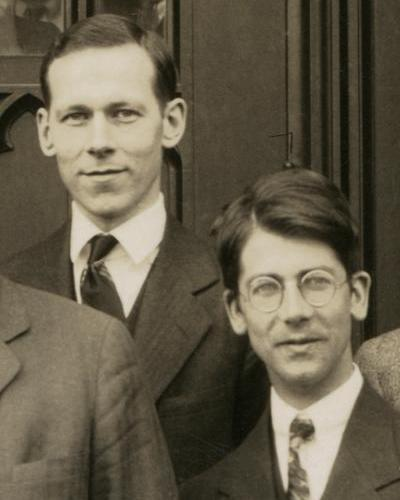
\includegraphics[width=\linewidth]{images/book3/mulliken-hund.jpg}
\end{minipage}\hfill
\begin{minipage}[t]{0.69\linewidth}
\vspace{0pt}
1926 年至 1932 年间，弗里德里希·洪特与罗伯特·马利肯通过
将每个电子归入整个分子的一条轨道来解释双原子分子的光谱，
这些轨道按其绕轴的对称性分类。“$\sigma$”、“$\pi$”、
成键与反键等词，以及本章的轨道图，都出自他们的
工作；马利肯于 1966 年获诺贝尔化学奖。照片展示的是 1929 年在芝加哥的
马利肯（左）与洪特。（照片：GFHund，CC BY 3.0，
维基共享资源。）
\end{minipage}
\end{history}

\section{电离与键强}

从成键轨道移去一个电子会削弱键；从
反键轨道移去一个电子则增强键。离子的解离能
可由热化学循环求得：对于 $\mathrm{AB}^+ \to \mathrm A + \mathrm B^+$，
\[
  D_0(\mathrm{AB}^+) = D_0(\mathrm{AB}) + I(\mathrm B) - I(\mathrm{AB}) ,
\]
其中 B 为电离能较低的原子。

\begin{example}[氮与氧的离子]\label{ex:b2:diatomic-mos:ions}
\ce{N2}（$I = \qty{15.58}{eV}$）失去一个成键电子：$D_0(\ce{N2+}) = 9.76 + 14.53 -
15.58 = \qty{8.71}{eV}$，弱于 \ce{N2}。\ce{O2}（$I = \qty{12.07}{eV}$）失去一个
$\pi^*$ 电子：$D_0(\ce{O2+}) = 5.12 + 13.62 - 12.07 = \qty{6.66}{eV}$，强于 \ce{O2}，
与键级 2.5 和 2.5 对比 3 和 2 相符。
% ledger: ie:N2, ie:N, ie:O2, ie:O, janafH0:N, janafH0:O
\end{example}

\section{练习}

\begin{exercise}[$\star$]\label{exo:b2:diatomic-mos:1}
对两个氢的 1s 轨道取 $\alpha = \qty{-13.6}{eV}$，$\beta = \qty{-9.0}{eV}$，
$S = 0.60$（练习数据）。求 $E_+$ 与 $E_-$，再求
\ce{H2} 中两个电子的能量，并与两个独立原子相比较。
\end{exercise}

\begin{exercise}[$\star$]\label{exo:b2:diatomic-mos:2}
求 \ce{He2}、\ce{He2+}、\ce{Li2} 与 \ce{B2} 的键级（考虑 s--p
混合）。
\end{exercise}

\begin{exercise}[$\star$]\label{exo:b2:diatomic-mos:3}
在 \ce{B2}、\ce{C2}、\ce{N2}、\ce{O2}、\ce{F2} 中，哪些是顺磁性的？
\end{exercise}

\begin{exercise}[$\star$]\label{exo:b2:diatomic-mos:4}
设分子轴为 $z$。在 (1s, $2\mathrm p_z$)、(1s,
$2\mathrm p_x$)、($2\mathrm p_x$, $2\mathrm p_x$)、($2\mathrm p_x$, $2\mathrm p_y$)、
(2s, $2\mathrm p_z$) 中，哪些对的重叠积分不为零？
\end{exercise}

\begin{exercise}[$\star\star$]\label{exo:b2:diatomic-mos:5}
判断 \ce{N2+} 的键比 \ce{N2} 更长还是更短，并用
本章计算出的解离能加以检验。
\end{exercise}

\begin{exercise}[$\star\star$]\label{exo:b2:diatomic-mos:6}
一氧化碳与 \ce{N2} 互为等电子体。试说明 CO 的
成键轨道为何偏向氧原子，以及其最高占据轨道为何是
碳上的孤电子对。
\end{exercise}

\begin{exercise}[$\star\star$]\label{exo:b2:diatomic-mos:7}
在 HF 中，氟的哪些轨道与氢的 1s 轨道相互作用，哪些
保持为非键轨道？画出能级图。
\end{exercise}

\begin{exercise}[$\star\star$]\label{exo:b2:diatomic-mos:8}
已知 $\alpha_A = \qty{-10}{eV}$，$\alpha_B = \qty{-14}{eV}$，$\beta = \qty{-3.0}{eV}$
（练习数据，忽略 $S$），计算两个能量及
成键轨道中 B 的权重 $c_B^2$。
\end{exercise}

\begin{exercise}[$\star\star$]\label{exo:b2:diatomic-mos:9}
考虑 s--p 混合，证明 \ce{C2} 的键级为 2，由两个 $\pi$ 键构成，且
不存在 $\sigma_{2p}$ 键。
\end{exercise}

\begin{exercise}[$\star\star\star$]\label{exo:b2:diatomic-mos:10}
求 NO 和 \ce{NO+} 的键级。由 $D_0(\ce{NO}) = \qty{6.51}{eV}$，$I(\ce{NO}) =
\qty{9.26}{eV}$ 和 $I(\ce{O}) = \qty{13.62}{eV}$，计算 $D_0(\ce{NO+})$，其中 $\ce{NO+} \to
\ce{N} + \ce{O+}$ 的过程，并加以评述。
\end{exercise}

\begin{exercise}[$\star\star\star$]\label{exo:b2:diatomic-mos:11}
证明 $E_+ + E_- = 2(\alpha - \beta S)/(1 - S^2)$，并证明它大于 $2\alpha$
（条件为 $\beta < \alpha S < 0$）。由此说明两个充满的
轨道为何相互排斥（四电子去稳定化）。
\end{exercise}

\begin{exercise}[$\star\star\star$]\label{exo:b2:diatomic-mos:12}
按键级、键长和键
强度对 \ce{O2+}、\ce{O2}、\ce{O2-}、\ce{O2^2-} 排序。过氧化氢中含有哪种离子，黄色的
化合物 \ce{KO2} 中含有哪种离子？
\end{exercise}

\section{问题：氧及其离子}

\begin{problem}[{周末问题——双原子氧的分子轨道能级图，
其离子的键级与磁性、电离及键强度，
以及 $\pi^*$ 电子的两种配对方式}]
\label{pb:b2:diatomic-mos:1}
数据：$I(\ce{O}) = \qty{13.62}{eV}$，$I(\ce{O2}) = \qty{12.07}{eV}$，$I(\ce{N}) =
\qty{14.53}{eV}$，$I(\ce{N2}) = \qty{15.58}{eV}$；$\Delta_f H_0$ 于 \qty{0}{K}
（\unit{kJ/mol}）：\ce{O} 246.79，\ce{N} 470.82；$r_e$：\ce{O2} \qty{120.8}{pm}，\ce{N2}
\qty{109.8}{pm}；$1\ \unit{eV} = \qty{96.485}{kJ/mol}$。
% ledger: ie:O, ie:O2, ie:N, ie:N2, janafH0:O, janafH0:N, re:O2, re:N2

\medskip
\noindent\textbf{第一部分——双原子氧。}
\begin{enumerate}
  \item \ce{O2} 有多少个价电子？
  \item 画出其价层分子轨道能级图（不考虑 s--p 混合）并填充电子。
  \item 计算其键级。
  \item 有多少个未成对电子？\ce{O2} 是否为顺磁性物质？
  \item 为何路易斯结构在此处失效？
  \item 以 \unit{eV} 为单位计算 $D_0(\ce{O2})$。
\end{enumerate}

\medskip
\noindent\textbf{第二部分——离子。}
\begin{enumerate}[resume]
  \item 给出 \ce{O2+} 的电子排布和键级。
  \item 对超氧离子 \ce{O2-} 做同样的计算。
  \item 对过氧离子 \ce{O2^2-} 做同样的计算。
  \item 给出各离子中未成对电子的数目。
  \item 按预测的键长对 \ce{O2+}、\ce{O2}、\ce{O2-}、\ce{O2^2-} 排序。
  \item 哪种离子含有与过氧化氢相同的 O--O 单键？
  \item 四种物种中哪些是顺磁性的？
\end{enumerate}

\medskip
\noindent\textbf{第三部分——电离。}
\begin{enumerate}[resume]
  \item \ce{O2} 电离时，电子从哪个轨道离开？
  \item 为何 $I(\ce{O2})$ 低于 $I(\ce{O})$？
  \item 证明 $D_0(\ce{O2+}) = D_0(\ce{O2}) + I(\ce{O}) - I(\ce{O2})$，并计算其值。
  \item 与 $D_0(\ce{O2})$ 相比较，并加以解释。
  \item 用同样的方法计算 $D_0(\ce{N2})$ 和 $D_0(\ce{N2+})$。
  \item 为何 $I(\ce{N2})$ 高于 $I(\ce{N})$？
  \item 总结：电离在何种情况下会增强键？
\end{enumerate}

\medskip
\noindent\textbf{第四部分——$\pi^*$ 电子。}
\begin{enumerate}[resume]
  \item 在基态中，两个 $\pi^*$ 电子占据两个不同的
        轨道，且自旋平行。哪条规则规定了这一点？
  \item 描述两个电子占据同一 $\pi^*$ 轨道的状态。
  \item 为何该状态的能量更高？
  \item 该状态的键级和磁性各是多少？
  \item 写出 \ce{O2+} 的键级及其解离能。
\end{enumerate}
\end{problem}
